%% -*- Mode: LaTeX -*-
%%
%% filexfer.tex
%% Created Mon Jun 27 09:39:25 AKDT 2016
%% by Raymond E. Marcil <rmarcil@gci.com>
%% 
%% FileXfer - File Transfer Jobs
%%
%% Links
%% =====
%% Creating Flowcharts with TikZ
%% ShareLaTeX Blog
%% https://www.sharelatex.com/blog/2013/08/29/tikz-series-pt3.html
%%


  %%
%%%%%% Preamble.
  %%

%% Specify DVIPS driver used by things like hyperref
\documentclass[12pt,letterpaper,dvips]{article}


%% rcs is the package to display cvs revision info.
%%\usepackage{rcs}
\usepackage{fullpage}
\usepackage{fancyvrb}

%% Decorative lines on header and footer
%% https://www.sharelatex.com/learn/Headers_and_footers
\usepackage{fancyhdr}

\usepackage{graphicx}
\usepackage{figsize}
\usepackage{calc}

%%
%% Use got bold \texttt
%% \texttt{TT Text \textbf{Bold TT Text}}
%%     or
%% \texttt{\textbf{foo}}
%%
%% How do I get \texttt with bold face in LaTeX?
%% http://tex.stackexchange.com/questions/215482/how-do-i-get-texttt-with-bold-face-in-latex
%%
\usepackage{bold-extra}

\usepackage{verbatim}

%%
%% LaTeX/Source Code Listings
%% https://en.wikibooks.org/wiki/LaTeX/Source_Code_Listings
%%
\usepackage{listings}

%% Tables that span multiple pages
\usepackage{longtable}

%%
%% enumitem – Control layout of itemize, enumerate, description
%% https://www.ctan.org/pkg/enumitem
%%
%% Allows for use of \bgein{itemize}[leftmargin=0pt] 
%% to lists with 0 left margin.
%%
%% Itemize left margin
%% http://tex.stackexchange.com/questions/170525/itemize-left-margin
%% 
\usepackage{enumitem}%     http://ctan.org/pkg/enumitem


%% caption package for use in justifying table or figure captions
\usepackage{caption}

\usepackage{xspace}
\usepackage{booktabs}
\usepackage[first,bottomafter]{draftcopy}
\usepackage[numbib]{tocbibind}

%%
%% Creating Flowcharts with TikZ
%% https://www.sharelatex.com/blog/2013/08/29/tikz-series-pt3.html
%%
\usepackage{tikz}
\usetikzlibrary{shapes.geometric, arrows}

\usepackage{amssymb}              %% AMS Symbols, used for \checkmark
\usepackage{multicol}

%%
%% Extract SVN metadata for use elsewhere.
%% This information has:
%% o the filename
%% o the revision number
%% o the date and time of the last Subversion co command
%% o name of the user who has done the action
%%
%% FIXME: Need to update this for git.
%%
%%\usepackage{svninfo}
%%\svnInfo $Id: filexfer.tex 52 2016-06-27 09:43:54Z marcilr $


%%
%% Including Git Revision Identifiers in LaTeX
%% by Thore Husfeldt
%% https://thorehusfeldt.net/2011/05/13/including-git-revision-identifiers-in-latex/
%% Configure git user name
%%   For individual repo:
%%     $ git config user.name "Bob Jones"
%%
%%   For all repos:
%%     $ git config --global user.name "Bob Jones"
%%
%% Verify user name for repo:
%%   $ git config user.name
%%   Bob Jones
%%
%% Verify user name all repos:
%%   $ git config --global user.name
%%   Bob Jones
%%
%% Changing your username in Git only affects commits that
%% you make after your change.
%%
%% To rewrite your old commits, you can use git filter-branch[1]
%% to change the repository history to use your new username.
%% [1] https://help.github.com/articles/changing-author-info
%%
%%% This file is generated by Makefile.
%%% Do not edit this file!
%%%
\gdef\GITAuthorEmail{marcilr@gmail.com}
\gdef\GITRevision{0.0.1}
	\gdef\GITAbrHash{c35cce8}	\gdef\GITAuthorDate{June 28, 2016}	\gdef\GITAuthorName{Raymond E. Marcil}

%%
%% Hyperref package for embedding URLs for clickable links in PDFs, 
%% also specify PDF attributes here.
%%
%% The pdfborder={0 0 0} is what ellimated the blue box around the url
%% displayed by \href{}{}.
%%
%% The command pdfborder={0 0 1} would display a box with thickness of 1 pt.
%%
%% Hypertext marks in LATEX: a manual for hyperref
%% by Sebastian Rahtz and Heiko Oberdiek - November 2012
%% http://ctan.org/pkg/hyperref 
%% http://mirror.hmc.edu/ctan/macros/latex/contrib/hyperref/doc/manual.html
%%
\usepackage[
colorlinks,
linkcolor=blue,
%%colorlinks=false,
hyperindex=false,
urlcolor=blue,
pdfborder={0 0 0},
pdfauthor={Raymond E. Marcil},
pdftitle={FileXfer File Transfer Jobs},
pdfcreator={ps2pdf},
pdfsubject={FileXfer, file transfer jobs},
pdfkeywords={FileXfer, file transfer jobs}
]{hyperref}


%%
%% Extract RCS metadata for use elsewhere.
%% Jason figured this out, very cool.
%%
%%\RCS $Revision: 1.53 $
%%\RCS $Date: 2006/06/26 21:04:55 $


  %%
%%%%%% Customization.
  %%

% On letter paper with 10pt font the Verbatim environment has 65 columns.
% With 12pt font the environment has 62 columns.  Exceeding this will exceed
% the frame and will look ugly.  YHBW.  HAND.
\RecustomVerbatimEnvironment{Verbatim}{Verbatim}{frame=single}

\renewenvironment{description}
                 {\list{}{\labelwidth 0pt \iteminden-\leftmargin
                          \let\labelsep\hsize
                          \let\makelabel\descriptionlabel}}
                 {\endlist}
\renewcommand*\descriptionlabel[1]{\hspace\labelsep\sffamily\bfseries #1}


  %%
%%%%%% Commands.
  %%

\newcommand{\FIXME}[1]{\textsf{[FIXME: #1]}}
\newcommand{\cmd}[1]{\texttt{#1}}


%% Squeeze space above/below captions
\setlength{\abovecaptionskip}{4pt}   % 0.5cm as an example
\setlength{\belowcaptionskip}{4pt}   % 0.5cm as an example


%% Tex really adds a lot of whitespace to itemized 
%% lists so define a new command itemize* with a 
%% lot less whitespace.  Found this in the British
%% Tex faq.
\newenvironment{itemize*}%
  {\begin{itemize}%
    \setlength{\itemsep}{0pt}%
    \setlength{\parsep}{0pt}}%
  {\end{itemize}}

  
%%
%% Tex really adds a lot of whitespace to itemized 
%% lists so define a new command itemize* with a 
%% lot less whitespace.  Found this in the British
%% Tex faq.
%%
%% Tue Jun 23 13:22:04 AKDT 2015
%% =============================
%% Added [leftmargin=0.0mm] to set the left margin=0
%% This requires use of the enumitem package:
%%   \usepackage{enumitem}%     http://ctan.org/pkg/enumitem
%%
%% Itemize left margin
%% http://tex.stackexchange.com/questions/170525/itemize-left-margin
%%
\newenvironment{itemizenoleft*}%
  {\begin{itemize}[leftmargin=15.0pt]%
    \setlength{\itemsep}{0pt}%
    \setlength{\parsep}{0pt}}%
  {\end{itemize}}
  

%%
%% Tex really adds a lot of whitespace to itemized 
%% lists so define a new command enumerate* with a 
%% lot less whitespace.  Created using itemize*
%% pattern.  
%%
  \newenvironment{enumerate*}%
  {\begin{enumerate}%
    \setlength{\itemsep}{0pt}%
    \setlength{\parsep}{0pt}}%
  {\end{enumerate}}


%%
%% Tex really adds a lot of whitespace to itemized 
%% lists so define a new command enumerate* with a 
%% lot less whitespace.  Created using itemize*
%% pattern.  
%%
%% Tue Jun 23 13:22:04 AKDT 2015
%% =============================
%% Added [leftmargin=0.0mm] to set the left margin=0
%% This requires use of the enumitem package:
%%   \usepackage{enumitem}%     http://ctan.org/pkg/enumitem
%%
%% Itemize left margin
%% http://tex.stackexchange.com/questions/170525/itemize-left-margin
%%
\newenvironment{enumeratenoleft*}%
  {\begin{enumerate}[leftmargin=0.0mm]%
    \setlength{\itemsep}{0pt}%
    \setlength{\parsep}{0pt}}%
  {\end{enumerate}}


%% Squeeze space
\renewcommand\floatpagefraction{.9}
\renewcommand\topfraction{.9}
\renewcommand\bottomfraction{.9}
\renewcommand\textfraction{.1}   
\setcounter{totalnumber}{50}
\setcounter{topnumber}{50}
\setcounter{bottomnumber}{50}

%%
%% The tikzstyle command
%% Now before we start the document we need to define the basic components of
%% a flow chart.  To do this we use the \tikzstyle command.  First let’s
%% define the block we’re going to use for start and stop blocks.  We’ll name
%% it ‘startstop’ using curly brackets immediately following the command, then
%% we add an equals sign before a set of square brackets. In the square
%% brackets we enter all the formatting information. For this block we’ll
%% specify a rectangle with rounded corners.  We’ll give it a minimum width of
%% 3cm and a minimum height of 1cm.  We’ll also ensure the text gets centred
%% and we’ll set both a draw and a fill colour.  In this example we’ve set the
%% fill colour to a colour that is 30% red mixed with 70% white.
%% --sharelatex.com/
%%
\tikzstyle{startstop} = [rectangle, rounded corners, minimum width=3cm,
  minimum height=1cm,text centered, draw=black, fill=red!30]

%%
%% Next we’ll specify an input or output box. This time we want the block to
%% be a parallelogram.  To achieve this we ask for a trapezium and then alter
%% the angles. The rest is very similar.
%% --sharelatex.com/
%%
\tikzstyle{io} = [trapezium, trapezium left angle=70, trapezium right
  angle=110, minimum width=3cm, minimum height=1cm, text centered, draw=black,
  fill=blue!30]

%%
%% Next we’ll add a TikZ style for process blocks using a rectangle and a
%% style for decision blocks using a diamond.
%% --sharelatex.com/
%%
\tikzstyle{process} = [rectangle, minimum width=3cm, minimum height=1cm, text centered, draw=black, fill=orange!30]
\tikzstyle{decision} = [diamond, minimum width=3cm, minimum height=1cm, text
  centered, draw=black, fill=green!30]

%%
%% Finally we’ll define a style for the arrows. For this we set the line
%% thickness to ‘thick’, add an arrow head and specify the stealth arrow head.
%% --sharelatex.com/
%%
\tikzstyle{arrow} = [thick,->,>=stealth]


%%
%% Decorative lines on header and footer
%% Headers and footers
%% https://www.sharelatex.com/learn/Headers_and_footers
%%
%% E for even page
%% O for odd page
%% L for left side
%% C for centered
%% R for right side
%%
\pagestyle{fancy}
\fancyhf{}
%%\fancyhead[CE,RO]{\leftmark}
\fancyhead[RE,LO]{FileXfer}
%% Center like 6 OPERATION
%%\fancyfoot[CE,CO]{\leftmark}
\fancyfoot[LE,RO]{\thepage}

%% FIXME: Need to get initial creation data and current branch here.
\lfoot{Created \GITAuthorDate\hspace{5pt}from \texttt{\jobname.tex}
  (sha-1: \texttt{\GITAbrHash})\\
  by \GITAuthorName \hspace{5pt}\texttt{$<$\GITAuthorEmail$>$}}



  %%
%%%%%% Document.
  %%

\title{FileXfer\\ File Transfer Jobs}

\author{\GITAuthorName\\
        \texttt{$<$\GITAuthorEmail$>$}
%%        \texttt{$<$rmarcil@gci.com$>$}
}

% Display subversion revision and date under author on 1st page.
%%\date{Revision \svnInfoRevision
%%      \hspace{2pt}
%%      (\svnInfoLongDate)}

%%
%% Including Git Revision Identifiers in LaTeX
%% Thore Husfelt
%% https://thorehusfeldt.net/2011/05/13/including-git-revision-identifiers-in-latex/
%%
\date{Revision \GITRevision\hspace{7.5pt}(\GITAuthorDate)}


%% ===================== Document ======================
%% ===================== Document ======================
%% ===================== Document ======================
\begin{document}


%%
%% Document sections
%% -----------------
%% Title
%% Abstract
%% Table of Contents
%% List of Figures
%% List of Tables
%% List of Abbreviations
%% Introduction
%% Design
%% Schema
%% Implementation
%% Operation
%% Appendix
%%
\maketitle
%% -*- Mode: LaTeX -*-
%%
%% abstract.tex
%% Created Fri Jul  1 09:15:38 AKDT 2016
%% by Raymond E. Marcil <rmarcil@gci.com>
%%
%% Abstract for file transfer jobs
%%


%% ===================== Abstract ======================
%% ===================== Abstract ======================
\begin{abstract}
  \noindent The FileXfer application is a system for automated file transfer
  jobs for copying files.  ``There are 3 applications that make up the usage
  collection framework: \texttt{filexfer}, which does the actual file
  transfers; \texttt{filexfer-jobmonitor}, which is configured
  to monitor various aspects of jobs and create NMS alarms when necessary; and
  \texttt{filexfer-}\\
  \texttt{dataloader}, which bulk-loads file data into database
  tables. There are also housekeeping scripts called
  \texttt{filexfer-filearchive}, which keeps files in the data directory
  pruned and compressed, and \texttt{filexfer-fileunarchive}, which allows
  files to be pulled out of the archive so filexfer jobs can work with them
  again.''\footnote{\href{http://oss-wiki.operations.gci.com/dev/index.php/Usage\_Collection\_Framework\_(filexfer)}{Usage Collection Framework (filexfer)}}
\end{abstract}

\vspace{2.0in}
\newpage
\tableofcontents
\newpage
\listoffigures
\listoftables
%% -*- Mode: LaTeX -*-
%%
%% list-of-abbreviations.tex
%% Created Fri Jul  1 09:02:36 AKDT 2016
%% by Raymond E. Marcil <rmarcil@gci.com>
%%
%% List of Abbreviation for file transfer jobs
%%

%% =============== List of Abbreviations ===============
%% =============== List of Abbreviations ===============
\newpage
\setcounter{secnumdepth}{0}
\section{List of Definitions and Abbreviations}
\begin{itemize*}
  \item{\begin{bf}MOA\end{bf}} - Municipality of Anchorage

\end{itemize*}

%% -*- Mode: LaTeX -*-
%%
%% introduction.tex
%% Created Fri Jul  1 08:53:27 AKDT 2016
%% by Raymond E. Marcil <rmarcil@gci.com>
%%
%% Introduction for file transfer jobs
%%



%% ====================== Introduction ===========================
%% ====================== Introduction ===========================
%% ====================== Introduction ===========================
\newpage
\setcounter{secnumdepth}{2}
\section{Introduction}
\fancyhead[LE,RO]{INTRODUCTION}
FileXfer is a custom application that GCI OSS built whose primary
purpose is to transfer files from point A to point B (most of the
time via point C/itself).  It can also be used to load the
collected data into a database if the data fits within the
constraints of MySQL Load Data Infile SQL Syntax.  It supports
FTP and SFTP for both gets and puts, and it also has limited
support for HTTP gets (this feature is used to collect weather
camera images off of the Terra mountain top sites for the
FAA).\footnote{FileXfer.txt:3, GCI Network Services, OSS Mark
Blum, Spring 2016}\\
\\
FileXfer can also be used to prune the source server's target
files to a certain number of days.  And while the default is
to keep the source file time, this feature can be toggle off
on a per job basis, resulting in the files having the transfer
time instead as some customers prefer to know when the file
was dropped off and not when the file was generated.  For
performance reasons there is a cutoff feature as well which
defaults to 5 days for new jobs.  FileXfer will not look more
than the cutoff days back to see if a file should be collected
and/or exported.  FileXfer jobs are also capable of running
in audit mode, in which FileXfer will log all of the transfers
but it won't physically transfer anything.  This feature can
be useful to get a feed caught up without transfering a bunch
of files around if for whatever reason the backlog of files
doesn't need to be processed by any customers.\\
\\
FileXfer logs all file transfers and any errors.  However, it
is not considered an error if there are no files to collect.
FileXfer also supports monitoring of transfer jobs, and can
generate an alert for any reason that you can articulate with
SQL.  Some examples include late and/or missing files, load
queue too large, file too small, no files transfered for a
certain interval, etc.  The monitoring supports internal
only alerts, TAC visibile alerts, and/or emailing the alerts.
The email feature also supports sending of texts to cell
phones.\\
\\
FileXfer will re-transfer a file if either the size and/or
source file time changes, as that signals something about the
file has changed.  Some feeds leverage this concept as they
may use a static filename in which the data is simply re-writen
to same exact file at regular intervals.\\
\\
The main FileXfer app server is
\texttt{prod-prov4-cdr1.operations.gci.com}
(\texttt{192.168.161.47}).  The ''ACS'' / Project Seward
FileXfer app server (which contains only ACS/Project
Serward related jobs) is the SPS2 OSS Test app server,
\texttt{osstest-em-provisioning.operations.gci.com}
(\texttt{192.168.56.4}; public IP \texttt{66.223.155.33}).



%% -*- Mode: LaTeX -*-
%%
%%
%% design.tex
%% Created Fri Jul  1 08:58:33 AKDT 2016
%% by Raymond E. Marcil <rmarcil@gci.com>
%%


%% ========================= Design ==============================
%% ========================= Design ==============================
%% ========================= Design ==============================
\newpage
\section{Design}
\fancyhead[LE,RO]{DESIGN}
\FIXME{Need data here...}

%%
%% TikZ flowchart
%% Plenty of notes on creating a TikZ flowchart.
%% Notes on making adjustable size boxes for arbitrary amount of text that I
%% did not use in this exmaple.
%% ShareLaTeX Blog
%% https://www.sharelatex.com/blog/2013/08/29/tikz-series-pt3.html
%% 
\vspace{2cm}
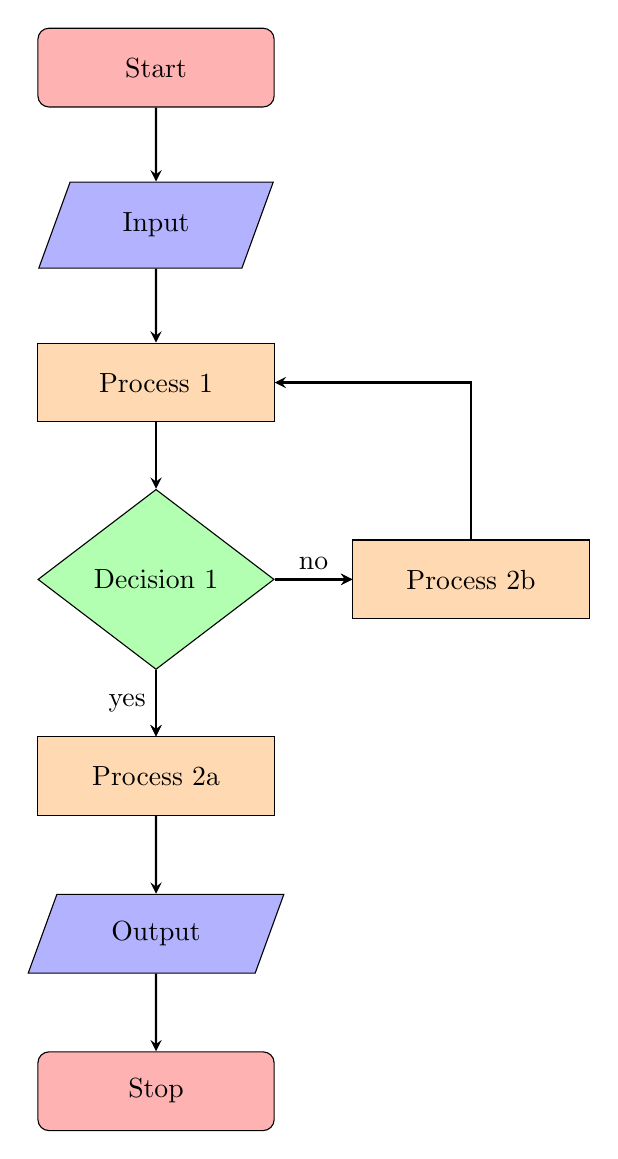
\begin{tikzpicture}[node distance=2cm]

  <TikZ code>

  %% Start block
  \node (start) [startstop] {Start};
  \node (in1) [io, below of=start] {Input};
  \node (pro1) [process, below of=in1] {Process 1};
%%  \node (dec1) [decision, below of=pro1] {Decision 1};
  \node (dec1) [decision, below of=pro1, yshift=-0.5cm] {Decision 1};

  \node (pro2a) [process, below of=dec1, yshift=-0.5cm] {Process 2a};
  \node (pro2b) [process, right of=dec1, xshift=2cm] {Process 2b};
  \node (out1) [io, below of=pro2a] {Output};
  \node (stop) [startstop, below of=out1] {Stop};


  \draw [arrow] (start) -- (in1);
  \draw [arrow] (in1) -- (pro1);
  \draw [arrow] (pro1) -- (dec1);
  \draw [arrow] (dec1) -- (pro2a);
  \draw [arrow] (dec1) -- (pro2b);

  \draw [arrow] (dec1) -- node[anchor=east] {yes} (pro2a);
  \draw [arrow] (dec1) -- node[anchor=south] {no} (pro2b);

  %% Makes diagonal line
%%  \draw [arrow] (pro2b) -- (pro1);

  %% Make the arrow go in a vertical direction before going in a horizontal
  %% direction.
  \draw [arrow] (pro2b) |- (pro1);
  
  \draw [arrow] (pro2a) -- (out1);
  \draw [arrow] (out1) -- (stop);
  
\end{tikzpicture}

\vspace{10pt}
\noindent \FIXME{Customize flowchart FileXfer}

%% -*- Mode: LaTeX -*-
%%
%% schema.tex
%% Created Fri Jul  1 08:37:02 AKDT 2016
%% by Raymond E. Marcil <rmarcil@gci.com>
%%
%% Schema used by file transfer jobs
%%

%% ========================= Schema ============================
%% ========================= Schema ============================
%% ========================= Schema ============================
\newpage
\section{Schema}
The main FileXfer database server is
\texttt{sadc-cdr-mysql1.operations.gci.com}
(\texttt{192.68.56.189}) and the ACS/Project Seward
FileXfer database server is the SPS2 OSS Test database
server, \texttt{osstest-db-provisioning.operations.gci.com}
(\texttt{192.168.69.149}).  For both database servers
the FileXfer database is called \texttt{filexfer}.\footnote{FileXfer.txt:11, GCI Network Services, OSS Mark Blum, Spring 2016}\\
\\
\noindent Here's a breakdown of the tables:
\begin{verbatim}
[mblum@development-mark ~]$ mysql -h sadc-cdr-mysql1 -sss \
-e "USE filexfer; SHOW TABLES"
DATABASECHANGELOG
DATABASECHANGELOGLOCK
errors
joblogs
jobs
loadjobs
loadqueue
logs
monitors

DATABASECHANGELOG
DATABASECHANGELOGLOCK

\end{verbatim}

\noindent These two tables manage how updates to the database structure
of FileXfer are preformed and stored.

\subsection{\texttt{errors}}
This table stores any errors FileXfer encounters.

\subsection{joblogs}
This is actually a view.  Here's the create statement:

\begin{verbatim}
CREATE 
    ALGORITHM = UNDEFINED 
    DEFINER = `filexfer`@`%` 
    SQL SECURITY DEFINER
VIEW `filexfer`.`joblogs` AS
    SELECT 
        `j`.`idJob` AS `idJob`,
        `l`.`idLog` AS `idLog`,
        `j`.`jobName` AS `jobName`,
        `j`.`neName` AS `neName`,
        `l`.`srcFileName` AS `srcFileName`,
        `l`.`srcFileSize` AS `srcFileSize`,
        `l`.`srcFileTime` AS `srcFileTime`,
        `l`.`destFileSize` AS `destFileSize`,
        `l`.`destFileName` AS `destFileName`,
        `l`.`dtTransferStart` AS `dtTransferStart`,
        `l`.`dtTransferStop` AS `dtTransferStop`
    FROM
        (`filexfer`.`jobs` `j`
    JOIN `filexfer`.`logs` `l` ON ((`j`.`idJob` = `l`.`idJob`)));
\end{verbatim}

\subsection{jobs}
This stores all of the transfer jobs.  Transfer jobs utilize a cron
like schedule, and their run policy can be set to schedule (i.e.
run as per the cron schedule), always, and never.  There is also
a wantSummary field that can be set to either yes or no.  Some
customers (mainly StarSolutions MSC Usage jobs) want summaries of
the transfer file (number of records etc.) and this feature
automatically generates that and transfer it along with the file.
Priority is another feature of the FileXfer system.  Given a limited
amount of resources you can set differing priority levels for jobs
(1 - 100 with 1 being the highest priority), so that jobs with
higher priorities get preference over lower priority jobs when
system resources are constrained.  Generally production jobs get
high priority (5) and lab/test jobs get low priority (100).\\
\\
The \texttt{neName} field, which stands for Network Element Name,
basically defines the directory where the files will be stored.
They are stored in \texttt{/data/usage/[neName]}.  Files are
automatically archived if they are older than 2 days (to
\texttt{/data/usage/[neName]/archive}), and archived files are
deleted if they are older than 30 days.  There is a script that
can be used to unarchive files (say for retransfer purposes)
called \texttt{/usr/bin/filexfer-fileunarchive}.  It takes a
file mask to unarchive and supports glob syntax.\\
\\
The \texttt{idSite} field is an incomplete feature and not
really used at this time.

\subsection{\texttt{loadjobs}}
This stores all of the load jobs.  Not every transfer job has
a corrisponding load job, and some transfer jobs may have more
than one load job.

\subsection{\texttt{loadqueue}}
This is the queue for the load jobs.  Entries in here have yet
to be loaded.  The loading is done in order.\\
\\
Here's a SQL query that can be used to view the loadqueue:

\begin{verbatim}
# FileXfer Load Queue Status
SELECT idJob, idLoadJob, jobName, neName,
IF( idJob = 0,FROM_UNIXTIME( Count ), Count ) AS 'Count', fileName, fileTime
FROM 
(
	SELECT 0 AS 'idJob', 0 AS 'idLoadJob', 'Current Time' AS 'jobName',
        'neName', UNIX_TIMESTAMP( NOW() ) AS 'Count', 'fileName', 'fileTime'

	UNION

	SELECT idJob, idLoadJob, jobs.jobName, jobs.neName, COUNT(*),
        fileName, fileTime
	FROM filexfer.loadqueue 
	JOIN filexfer.loadjobs USING ( idLoadJob )
	JOIN filexfer.jobs USING ( idJob )
	GROUP BY `idJob`
	ORDER BY ( CASE WHEN `idJob` = 0 THEN 0 ELSE 1 END ) ASC, 5 DESC 
) x;
\end{verbatim}


\subsection{\texttt{logs}}
This is the table where all of the transfer logs are kept.
In order to retransfer a specific file that has not changed
you will have to delete the corrisponding log entry.  Log
entries are never pruned from this table.

\subsection{\texttt{monitors}}
This table encompasses all of the job monitors.  Like load
jobs, not every transfer job has a job monitor, and some
transfer jobs may have more than one job monitor.

%% -*- Mode: LaTeX -*-
%%
%% implementation.tex
%% Created Fri Jul  1 08:27:00 AKDT 2016
%% by Raymond E. Marcil <rmarcil@gci.com>
%%



%% ===================== Implementation  =========================
%% ===================== Implementation  =========================
%% ===================== Implementation  =========================
\newpage
\section{Implementation}
\fancyhead[LE,RO]{IMPLEMENTATION}
\FIXME{Need data here...}


%%
%% Implementation subsection
%% -------------------------
%% Dependencies
%% Configuration
%% Scripts
%% Userscripts
%% Logging
%% Test
%% Issues
%%
%% -*- Mode: LaTeX -*- 
%%
%% dependencies.tex
%% Created Fri Jul  1 09:45:45 AKDT 2016
%% by Raymond E. Marcil <rmarcil@gci.com>
%%
%% Dependencies of file transfer jobs
%%


%% ======================== Dependencies =========================
%% ======================== Dependencies =========================
\subsection{Dependencies}

\begin{itemize}
    \item{cron}
    \item{inotify}
    \item{Perl v5.8.8}
    \item{Relevance}
\end{itemize}

%% -*- Mode: LaTeX -*- 
%%
%% configuration.tex
%% Created Fri Jul  1 09:31:16 AKDT 2016
%% by Raymond E. Marcil <rmarcil@gci.com>
%%
%% Configuration of file transfer jobs
%%


%% ======================= Configuration =========================
%% ======================= Configuration ========================= 
\subsection{Configuration}

\texttt{prod-prov4-cdr1}:
\begin{itemize}
    \item{\texttt{/etc/cron.d/filexfer}}
    \item{\texttt{/etc/cron.d/filexfer-userscripts}}
\end{itemize}

%% -*- Mode: LaTeX -*-
%%
%% relevance.tex
%% Created Thu Aug 11 08:34:36 AKDT 2016
%% by Raymond E. Marcil <rmarcil@gci.com>
%%
%% Relevance online interface
%%


%% ======================== Relevance ============================
%% ======================== Relevance ============================
%% ======================== Relevance ============================
\subsection{Relevance}
\FIXME{Need data here}

%% -*- Mode: LaTeX -*-
%%
%% scripts.tex
%% Created Fri Jul  8 15:38:16 AKDT 2016
%% Copyright (C) 2016 by Raymond E. Marcil <marcilr@gmail.com>
%%
%% Scripts
%%

\newpage
\subsection{Scripts}
The FileXfer application is made up of serveral scripts which are driven
by \texttt{cron} as follows:\footnote{FileXfer.txt:93, GCI Network Services,
OSS Mark Blum, Spring 2016}

\begin{verbatim}
[root@prod-prov4-cdr1 ~]# cat /etc/cron.d/filexfer
MAILTO=""
PERL5LIB=/opt

# This script preforms all of the get/collect jobs.
* * * * * filexfer /usr/bin/filexfer -c /etc/filexfer/filexfer-get.conf -t get
# This script preforms all of the put/export jobs.
* * * * * filexfer /usr/bin/filexfer -c /etc/filexfer/filexfer-put.conf -t put

# This script runs all of the job monitor jobs, and generates the relevant \
alerts and/or emails.
* * * * * filexfer /usr/bin/filexfer-jobmonitor -c /etc/filexfer/jobmonitor.conf

# This script runs all of the data loader jobs.
* * * * * filexfer /usr/bin/filexfer-dataloader -c /etc/filexfer/dataloader.conf
#* * * * * filexfer /usr/bin/filexfer-epg-dataloader.plx \
-c /etc/filexfer/epg-dataloader.conf

# These scripts take care of the archiving
2 0 * * * filexfer for dir in /data/usage/*; do /usr/bin/filexfer-filearchive \
$dir >>/var/log/filexfer/filearchive.log 2>&1; done
5 0 * * * filexfer find /data/usage -type f -name \*.sum -mmin +43200 | xargs rm
\end{verbatim}

\input{implementation/userscripts/userscripts.tex}
%% -*- Mode: LaTeX -*- 
%%
%% logging.tex
%% Created Fri Jul  1 11:04:13 AKDT 2016
%% by Raymond E. Marcil <rmarcil@gci.com>
%%
%% Logging
%%


%% ========================= Logging ===========================
%% ========================= Logging ===========================
\subsection{Logging}


%%
%% Logging sections
%% ----------------
%% Application Logging
%% File Transfer Logging
%%
%%
%% -*- Mode: LaTeX -*- 
%%
%% application-logging.tex
%% Created Fri Jul  1 11:07:46 AKDT 2016
%% by Raymond E. Marcil <rmarcil@gci.com>
%%
%% Application Logging
%%

%% ================== Application Logging ======================
%% ================== Application Logging ======================
\subsubsection{Application Logging}
The filexfer applications log to the \texttt{/var/log/filexfer}
directory on \texttt{prod-prov4-cdr1.}\textbackslash\\
\texttt{operations.gci.com}. The parent \texttt{filexfer} jobs
log to \texttt{filexfer-get.log} and
\texttt{filexfer-}\textbackslash\\
\texttt{put.log}.
The \texttt{jobmonitor} and \texttt{dataloader} applications
log to \texttt{jobmonitor.log} and\\
\texttt{dataloader.log}, The \texttt{filexfer} applications
log to the \texttt{/var/log/filexfer} directory on
\texttt{prod-prov4-cdr1.operations.gci.com}. The parent
\texttt{filexfer} jobs
log to \texttt{filexfer-get.}\textbackslash\\
\texttt{log} and \texttt{filexfer-put.log}. The
\texttt{jobmonitor} and \texttt{dataloader} applications log to\\
\texttt{jobmonitor.log} and \texttt{dataloader.log}, respectively. Each file
transfer job is executed as a child process and gets its own log file. The
format is\\
\texttt{filexfer-}$\{$\texttt{neName}$\}$\texttt{-}$\{$\texttt{idJob}$\}$\texttt{-}$\{$\texttt{get,put}$\}$\texttt{.log}.\\
\\
By default, the jobs log at the warn level.  Adjust the level to info to get a
high-level view of the application's state.  Adjust log verbosity by modifying
the appropriate config file in \texttt{/etc/filexfer}.  The changes will take
effect after the next program execution.\\
\\
Errors are also logged to a database table which can be browsed in the
filexfer web interface under the '\texttt{Logs \& Errors}' view.  This view
includes messages logged at \texttt{warn}, \texttt{error}, and \texttt{fatal}
severity.\footnote{\href{http://oss-wiki.operations.gci.com/dev/index.php/Usage\_Collection\_Framework\_(filexfer)}{Usage Collection Framework (filexfer)}}


%% -*- Mode: LaTeX -*- 
%%
%% file-transfer-logging.tex
%% Created Fri Jul  1 11:09:31 AKDT 2016
%% by Raymond E. Marcil <rmarcil@gci.com>
%%
%% File Transfer Logging
%%



%% ================= File Transfer Logging =====================
%% ================= File Transfer Logging =====================
\subsubsection{File Transfer Logging}
Every file transfer is recorded in a database table. There are
two reasons for this table: first, it tells \texttt{filexfer}
hich files have already been transferred, and second, it
provides an audit trail for SOX compliance. The table is
\texttt{filexfer.logs} on
\texttt{sadc-cdr-mysql1.operations.gci.com}. Use the
\texttt{filexfer.joblogs} view to easily find logs by job name
or network element ID.\\
\\
File transfer logs may also be viewed in the
'\texttt{Logs \& Errors}' page of the web
interface.\footnote{\href{http://oss-wiki.operations.gci.com/dev/index.php/Usage\_Collection\_Framework\_(filexfer)}{Usage
    Collection Framework (filexfer)}}


%% -*- Mode: LaTeX -*- 
%%
%% test.tex
%% Created Fri Jul  1 11:13:16 AKDT 2016
%% by Raymond E. Marcil <rmarcil@gci.com>
%%
%% Test
%%

%% =========================== Test ==============================
%% =========================== Test ==============================
\newpage
\subsection{Test}
\fancyhead[LE,RO]{TEST}
\FIXME{Need data here...}

%% -*- Mode: LaTeX -*- 
%%
%% issues.tex
%% Created Fri Jul  1 11:16:09 AKDT 2016
%% by Raymond E. Marcil <rmarcil@gci.com>
%%
%% Issues
%%


%% ========================== Issues =============================
%% ========================== Issues  ============================
\newpage
\subsection{Issues}
\fancyhead[LE,RO]{ISSUES}
\FIXME{Need data here...}



%% -*- Mode: LaTeX -*-
%%
%% operation.tex
%% Created Fri Jul  1 08:41:29 AKDT 2016
%% by Raymond E. Marcil <rmarcil@gci.com>
%%
%% Operation of file transfer jobs
%%

%% ======================== Operation ============================
%% ======================== Operation ============================
%% ======================== Operation ============================
\newpage
\section{Operation}
\fancyhead[LE,RO]{OPERATION}

There is a FileXfer GUI app on Relevance that can be used to
create/delete/update transfer/load jobs and monitors, and view
logs and errors.  It is available on both presenter 4 on
presenter 1 (but at this time it is safer to use presenter 4 to
update jobs). Also the lab presenter (lab-presenter4) is
currently pointed at the production ACS FileXfer
instance.\footnote{FileXfer.txt:149, GCI Network Services,
OSS Mark Blum, Spring 2016}\\


%%
%% Document sections
%% -----------------
%% FileXfer
%% Job Scheduling
%% Job Monitoring
%% Dataloader
%% Relevance
%%
%% -*- Mode: LaTeX -*-
%%
%% filexfer.tex
%% Created Mon Aug 22 10:20:54 AKDT 2016
%% by Raymond E. Marcil <rmarcil@gci.com>
%%
%% Filexfer
%%

%% ======================== FileXfer ============================
%% ======================== Filexfer ============================
%% ======================== Filexfer ============================
\subsection{FileXfer}
\fancyhead[LE,RO]{OPERATION}

There are times it is desirable to run FileXfer outside of the
FileXfer GUI app on Relevance.  Perhaps when it is desirable to
execute a single file transfer job. To do this login to 
GCI Network Services, OSS \texttt{prod-prov4-cdr1.operations.gci.com}
(\texttt{192.168.161.47}).\\
\\
The \texttt{filexfer} command is available from the command line.
It has relative straightforward syntax:

\begin{verbatim}
[root@prod-prov4-cdr1 usage]# /usr/bin/filexfer
Usage:
    filexfer.plx -c configfile -t {get|put} [options]

[root@prod-prov4-cdr1 usage]# cd ~
[root@prod-prov4-cdr1 ~]# /usr/bin/filexfer
Usage:
    filexfer.plx -c configfile -t {get|put} [options]

[root@prod-prov4-cdr1 ~]# /usr/bin/filexfer --help
Usage:
    filexfer.plx -c configfile -t {get|put} [options]

Arguments:
    -c, --configfile
        Specify the configuration file to load. Must be in YAML format.

    -t, --transfertype
        One of "get" or "put". Get jobs download files and put jobs upload
        files.

Options:
    -d, --piddir
        Directory where the pid file will be written. Defaults to
        /var/run/filexfer.

    --db
        Sets the database connection parameters. Valid keys are: server
        (default localhost), port (default 3306), driver (default mysql),
        uid, pwd, database, and table. Specify tags as key/value pairs,
        e.g.:

            --db server=localhost --db database=filexfer

    -e, --evengehost
        Address of the Evenge web server. Used to send indicators and events
        to the NMS system.

    --evengetimeout
        Timeout in seconds for communicating with the Evenge web server.
        Defaults to 10.

    -f, --cachefile
        Template cache file location. Defaults to
        /var/lib/filexfer/filexfer.kch.

    -h, --help
        Output this documentation.

    -m, --maxchildren
        Maximum number of child processes to spawn. Defaults to 50.

    -p, --pidfile
        PID file name. This will be appended with a ".pid" suffix.

    -r, --resource
        Resource name of this application. Used in indicator and event
        messages sent to the NMS system.

    --verbose, -v
        Log to the screen at increasingly verbose levels. This option may be
        repeated multiple times to increase the log level. For example, "-v"
        logs at info level, "-vv" logs at debug level, and "-vvv" logs at
        trace level.

[root@prod-prov4-cdr1 ~]# 
\end{verbatim}

\noindent The files transfered \texttt{filexfer} are under the
\texttt{/data/usage/} directory.

\begin{verbatim}
$ ssh hnmadm@prod-prov4-cdr1
hnmadm@192.168.161.47's password: 
Last login: Fri Aug 19 15:36:27 2016 from 10.103.193.217
[hnmadm@prod-prov4-cdr1 ~]$ cd /data/usage/
[hnmadm@prod-prov4-cdr1 usage]$ ls
AAA01       GA05  GA23  GA44  GA68  GC28  GC50    HAR01    P810     SPB02
ACS01       GA06  GA24  GA45  GA71  GC30  GC51    HCR01    P811     SPS02
AUB01       GA07  GA26  GA46  GA73  GC31  GC52    HMSC01   RBB01    SWPP01
BAL01       GA08  GA27  GA47  GA76  GC34  GC66    INC01    reports  SYNIVERSE
CAR01       GA09  GA28  GA48  GA77  GC35  GC87    INC02    RXNET01  TAL01
CBM01       GA10  GA29  GA49  GC05  GC36  GC88    INC03    SADC5E   TCS01
CDMA        GA11  GA30  GA50  GC15  GC37  GC89    IOP01    SBC01    TMP01
cdrReports  GA12  GA32  GA51  GC16  GC38  GC90    KUL01    SDC5E    TSUNAMI
CON01       GA13  GA33  GA52  GC17  GC39  GC91    legacy   SDE01    UNG01
CSKY01      GA14  GA34  GA53  GC18  GC41  GC93    LGCBX01  SDE01L   UNK01
CSKY02      GA15  GA35  GA55  GC19  GC42  GC94    MSW01    SDE01P   VORTEX01
DIM01       GA16  GA36  GA56  GC20  GC43  GC95    MTAS01   SDE02    WIFI01
EOS01       GA17  GA37  GA57  GC21  GC44  GC97    MUK01    SDE02L   WISP01
EPG01       GA18  GA38  GA58  GC22  GC45  GC98    Nov-18   SDE02P   WPS01
EPG02       GA19  GA39  GA59  GC23  GC46  GCT1    NRTRADE  SGSN01
GA01        GA20  GA41  GA65  GC24  GC47  GCT2    OCR01    SHU01
GA03        GA21  GA42  GA66  GC26  GC48  GGSN01  OSS01    SMSC01
GA04        GA22  GA43  GA67  GC27  GC49  GSM     P8       SPB01
[hnmadm@prod-prov4-cdr1 usage]$ sudo -s
Password:
[root@prod-prov4-cdr1 archive]#

\end{verbatim}

\noindent The directory names under \texttt{/data/usage/} map to the
\texttt{neName} column in the \texttt{filexfer.jobs} table that
is displayed in the FileXfer GUI application under the
File Transfer Jobs display in the \texttt{NE ID} field.\\
\\
The \texttt{filexfer get} jobs currently executing can be inspected with:

\begin{verbatim}
[root@prod-prov4-cdr1 usage]# ps ax | grep get
17585 ?        S      0:00 /usr/bin/filexfer \
-c /etc/filexfer/filexfer-get.conf -t get P8
17586 ?        S      0:00 /usr/bin/filexfer \
-x /etc/filexfer/filexfer-get.conf -t get P811
17588 ?        SN     0:00 /usr/bin/filexfer \
-c /etc/filexfer/filexfer-get.conf -t get SMSC01
17593 ?        SN     0:00 /usr/bin/filexfer \
-c /etc/filexfer/filexfer-get.conf -t get KUL01
17594 ?        SN     0:00 /usr/bin/filexfer \
-c /etc/filexfer/filexfer-get.conf -t get CAR01
24286 ?        S      0:00 /usr/bin/filexfer \
-c /etc/filexfer/filexfer-get.conf -t get GCT2
[root@prod-prov4-cdr1 usage]#
\end{verbatim}

\noindent The \texttt{filexfer put} jobs currently executing can be
inspected with:

\begin{verbatim}
[root@prod-prov4-cdr1 usage]# ps ax | grep put
...
 3863 ?        S      0:00 /usr/bin/filexfer \
-c /etc/filexfer/filexfer-put.conf -t put GC93
 3864 ?        S      0:00 /usr/bin/filexfer \
-c /etc/filexfer/filexfer-put.conf -t put GC94
 3866 ?        S      0:00 /usr/bin/filexfer \
-c /etc/filexfer/filexfer-put.conf -t put GC37
 3867 ?        S      0:00 /usr/bin/filexfer \
-c /etc/filexfer/filexfer-put.conf -t put GC95
 3869 ?        S      0:00 /usr/bin/filexfer \
-c /etc/filexfer/filexfer-put.conf -t put GA32
 3870 ?        S      0:00 /usr/bin/filexfer \
...
[root@prod-prov4-cdr1 usage]#
\end{verbatim}

\newpage
\noindent The same filexfer syntax displayed in the process list
can be using to execute an individual job to transfer files:

\begin{verbatim}
[root@prod-prov4-cdr1 ~]# /usr/bin/filexfer
Usage:
    filexfer.plx -c configfile -t {get|put} [options]

[root@prod-prov4-cdr1 ~]


[root@prod-prov4-cdr1 ~]# /usr/bin/filexfer -c /etc/filexfer/filexfer-put.conf -t put GC34
\end{verbatim}

%% -*- Mode: LaTeX -*-
%%
%% job-scheduling.tex
%% Created Thu Aug 11 08:10:02 AKDT 2016
%% by Raymond E. Marcil <rmarcil@gci.com>
%%
%% Job Scheduling in FileXfer
%%

%% ====================== Job Scheduling =========================
%% ====================== Job Scheduling ========================= 
%% ====================== Job Scheduling ========================= 
\subsection{Job Scheduling}
Jobs are scheduled using a web interface at
\texttt{nms.operations.gci.com/relevance}.  Navigate to the
``FileXfer'' application and click the ``File Transfer Jobs'' link.
Job execution happens on \texttt{prod-prov4-cdr1.operations.gci.com}.
A \texttt{cron} job executes every minute from
\texttt{/etc/cron.d/filexfer} to kick off the various \texttt{filexfer}
scripts.\footnote{\href{http://oss-wiki.operations.gci.com/dev/index.php/Usage\_Collection\_Framework\_(filexfer)}{Usage
    Collection Framework (filexfer)}}


%%
%% Document sections
%% -----------------
%% New Job
%% Job Timing
%% 
%% -*- Mode: LaTeX -*-
%%
%% new-job.tex
%% Created Thu Aug 11 08:15:46 AKDT 2016
%% by Raymond E. Marcil <rmarcil@gci.com>
%%
%% The basic requirements for setting up a new file transfer job.
%%

%% ===================== New Job =================================
%% ===================== New Job =================================
\subsubsection{New Job}
\noindent The basic requirements for setting up a transfer new job
are as follows:.\footnote{FileXfer.txt:139, GCI Network Services,
OSS Mark Blum, Spring 2016}\\
POC: [for when problems occur]\\
IP: [source host for collect jobs/destination host for export jobs]\\
Protocol: [ftp/sftp]\\
Credentials: [username/password]\\
File Path:\\
File Mask: [supports glob syntax]\\
Schedule: [cron syntax]\\
Want Summary: [yes/no; generally only for StarSolutions CDR exports]

%% -*- Mode: LaTeX -*-
%%
%% job-timing.tex
%% Created Thu Aug 11 08:15:46 AKDT 2016
%% by Raymond E. Marcil <rmarcil@gci.com>
%%
%% Job Timing for file transfer jobs
%%


%% =================== Job Timing ================================
%% =================== Job Timing ================================
\subsubsection{Job Timing}
The parent \texttt{filexfer} script is responsible for spawning
child processes for each job. Since a large number of jobs can be
scheduled at any given interval, the parent process limits how
many children can run concurrently.  As long as the limit is
reached and more jobs need to be spawned, the parent process must
stay alive. Since this may take longer than 1 minute, it is
possible for \texttt{filexfer} to miss certain scheduling
intervals.\\
\\
For example, if 500 jobs are scheduled to run at the top of every
hour \texttt{(0 * * * *)} and the maximum child process limit is
50, there is a good chance \texttt{filexfer} will not execute any
jobs scheduled to run at 1 minute past the hour
\texttt{(1 * * * *)}.  The best way to avoid this is to use
\texttt{0}, \texttt{15}, \texttt{30}, or \texttt{45} in the
minute field of the job schedule.  These intervals are always
executed.\footnote{\href{http://oss-wiki.operations.gci.com/dev/index.php/Scheduling\_Usage\_Collection\_Jobs}{Job
    Timing}}



%% -*- Mode: LaTeX -*-
%%
%% job-monitoring.tex
%% Created Thu Aug 11 07:59:59 AKDT 2016
%% by Raymond E. Marcil <rmarcil@gci.com>
%%
%% Job Monitoring of FileXfer
%%


%% ====================== Job Monitoring =======================
%% ====================== Job Monitoring =======================
\subsection{Job Monitoring}
The Relevance based FileXfer software has a Job Monitors section
where Email notifications can be configured.

%% -*- Mode: LaTeX -*-
%%
%% dataloader.tex
%% Created Thu Aug 11 08:26:49 AKDT 2016
%% by Raymond E. Marcil <rmarcil@gci.com>
%%
%% Dataloader jobs for FileXfer
%%


%% ======================= Dataloader ==========================
%% ======================= Dataloader ==========================
%% ======================= Dataloader ==========================
\subsection{Dataloader}
Dataloader jobs are configured using the web interface at
\texttt{nms.operations.gci.com/relevance}. Navigate to the
``\texttt{FileXfer}'' application and click the
``\texttt{Data Load Jobs}'' link. These jobs are executed every
minute as long as there are files in the load queue.\footnote{\href{http://oss-wiki.operations.gci.com/dev/index.php/Usage\_Collection\_Framework\_(filexfer)}{Usage Collection Framework (filexfer)}}

%% -*- Mode: LaTeX -*-
%%
%% relevance.tex
%% Created Thu Aug 11 08:34:36 AKDT 2016
%% by Raymond E. Marcil <rmarcil@gci.com>
%%
%% Relevance online interface
%%


%% ======================== Relevance ============================
%% ======================== Relevance ============================
%% ======================== Relevance ============================
\subsection{Relevance}
\FIXME{Need data here}


%% -*- Mode: LaTeX -*-
%%
%% appendix.tex
%% Created Fri Jul  1 08:47:41 AKDT 2016
%% Copyright (C) 2016 by Raymond E. Marcil <marcilr@gmail.com>
%%
%% Appendix for file transfer jobs
%%



%% ======================== Appendix =============================
%% ======================== Appendix =============================
%% ======================== Appendix =============================
%%
%% This will add a standard non-numbered Appendix to the document.
%% The next section Appendix changes secnumdepth such that the Appendix
%% is not numbered but still displayed in the table of contents (TOC).
%%
%% Adding unnumbered sections to TOC
%% http://tex.stackexchange.com/questions/11668/adding-unnumbered-sections-to-toc
%% 
%% \section*{Appendix}
%% Need content here.
%%
\newpage
\setcounter{secnumdepth}{0}
\section{Appendix}
\fancyhead[LE,RO]{APPENDIX}


%% ========================= Source ==============================
%% ========================= Source ==============================
\subsection{Source}
There are 3 primary FileXfer \texttt{perl} scripts on
\texttt{prod-prov4-cdr1}:\footnote{\texttt{prod-prov4-cdr1.operations.gci.com}
  (\texttt{192.168.161.47}, NATed IP: \texttt{66.223.199.228}), data including
  CDRs and such under \texttt{/data/usage/} ---
  Network Services, OSS.}


\begin{table}[htb]
\begin{tabular}{|p{.35\textwidth}|p{.17\textwidth}|p{.50\textwidth}|}\hline 
\textbf{File name}&\textbf{Attributes}&\textbf{Description}\\ 
\hline
\texttt{filexfer.plx}&181 lines&File transfer jobs\\
\texttt{filexfer-dataloader.plx}&132 lines&Data loader\\
\texttt{filexfer-jobmonitor.plx}&132 lines&Job Monitor\\
\hline
\end{tabular}
\caption{FileXfer \texttt{perl} scripts on \texttt{prod-prov4-cdr1}}
\label{table:FileXfer_scripts_on_prod-prov4-cdr1}
\end{table}


%% ====================== filexfer.plx ===========================
%% ====================== filexfer.plx ===========================
\newpage
\fancyhead[RE,LO]{\texttt{filexfer.plx}}
\fancyhead[CE,CO]{File Transfer Jobs}
\fancyhead[LE,RO]{APPENDIX}
\subsubsection{\texttt{filexfer.plx} --- File Transfer Jobs}

%%
%% Including a file verbatim in LaTeX
%% A good way is to use Rainer Schöpf’s verbatim package,
%% which provides a command \verbatiminput that takes a
%% file name as argument:
%%
%%     usepackage{verbatim}
%%     ...
%%     \verbatiminput{verb.txt}
%%
%% Including a file verbatim in LaTeX
%% http://www.tex.ac.uk/FAQ-verbfile.html
%%
%%\verbatiminput{./filexfer.plx}
%%\lstset{numbers=left}
\lstset{
    numbers=left,
    breaklines=true,
    postbreak=\raisebox{0ex}[0ex][0ex]{\ensuremath{\color{red}\hookrightarrow\space}}
}
\lstinputlisting{./appendix/source/filexfer.plx}


%% ================ filexfer-jobmonitor.plx ======================
%% ================ filexfer-jobmonitor.plx ======================
\newpage
\fancyhead[RE,LO]{\texttt{filexfer-jobmonitor.plx}}
\fancyhead[CE,CO]{Job Monitor}
\fancyhead[LE,RO]{APPENDIX}

\subsubsection{\texttt{filexfer-jobmonitor.plx} --- Job monitor}
%%\verbatiminput{./filexfer-jobmonitor.plx}

%%
%% lstlisting line wrapping
%% Great stuff.
%% http://tex.stackexchange.com/questions/116534/lstlisting-line-wrapping
%%
\lstset{
    numbers=left,
    breaklines=true,
    postbreak=\raisebox{0ex}[0ex][0ex]{\ensuremath{\color{red}\hookrightarrow\space}}
}
\lstinputlisting{./appendix/source/filexfer-jobmonitor.plx}


%% ================ filexfer-dataloader.plx ======================
%% ================ filexfer-dataloader.plx ======================
\newpage
\fancyhead[RE,LO]{\texttt{filexfer-dataloader.plx}}
\fancyhead[CE,CO]{Data Loader}
\fancyhead[LE,RO]{APPENDIX}

\subsubsection{\texttt{filexfer-dataloader.plx} --- Data Loader}
%%\verbatiminput{./filexfer-dataloader.plx}
\lstset{
    numbers=left,
    breaklines=true,
    postbreak=\raisebox{0ex}[0ex][0ex]{\ensuremath{\color{red}\hookrightarrow\space}}
}
\lstinputlisting{./appendix/source/filexfer-dataloader.plx}


\vspace{20pt}
\noindent\FIXME{Need data here}

\begin{longtable}[l]{ll}
%%    \label{FileXfer directories and files on prod-prov4-cdr1}
    \multicolumn{2}{c}%
    {{\bfseries \tablename\ \thetable{} -- FileXfer directories and files on \texttt{prod-prov4-cdr1}}} \\
    \hline
    \multicolumn{1}{|l|}{\textbf{Directory}} &
    \multicolumn{1}{l|}{\textbf{File(s)}}\\
    \hline
\endfirsthead

\multicolumn{2}{c}%
{{\bfseries \tablename\ \thetable{} -- continued from previous page}} \\
\hline
\multicolumn{1}{|l|}{\textbf{Directory}} &
\multicolumn{1}{l|}{\textbf{File(s)}} \\ \hline 
\endhead

\hline \multicolumn{2}{|r|}{{Continued on next page}} \\ \hline
\endfoot

%% This was double horizontal lines at end of table (removed)
%%\hline \hline
\endlastfoot

    \texttt{/etc/filexfer/}&\texttt{*.conf}\\
    \texttt{/usr/bin/}&\texttt{filexfer-dataloader}\\
    &\texttt{\textbf{filexfer-dataloader.plx}}\\
    &\texttt{filexfer-dataloader.plx.mbak}\\
    &\texttt{filexfer-epg-dataloader.plx}\\
    &\texttt{filexfer-filearchive}\\
    &\texttt{filexfer-filearchive.sh}\\
    &\texttt{filexfer-fileunarchive}\\
    &\texttt{filexfer-fileunarchive.sh}\\
    &\texttt{filexfer-jobmonitor}\\
    &\texttt{\textbf{filexfer-jobmonitor.plx}}\\
    &\texttt{\textbf{filexfer.plx}}\\
    \texttt{/usr/lib/filexfer}/&\texttt{*.gz, *.sh, *.plx}\\
    &\texttt{ExtractCarrierTurboZoneUsage*}\\
    \texttt{/usr/share/filexfer}/&\texttt{filexfer.changelog-*.xml}\\
    &\texttt{filexfer.changelog-master.xml}\\
    &\texttt{liquibase.sh}\\
    &\texttt{.gnupg/pubring.gpg}\\
    &\texttt{.gnupg/random\_seed}\\
    \texttt{/var/cache/yum/build/packages/}&\texttt{filexfer-0.52-1.el5.centos.noarch.rpm}\\
    \texttt{/var/lib/filexfer/}
    &\texttt{dataloader.kch}\\
    &\texttt{dataloader\_temp.kch}\\
    &\texttt{filexfer-aaa01-13-get.kch}\\
    &\texttt{...}\\
    &\texttt{filexfer-wps01-706-get.kch}\\
    &\texttt{filexfer.kch}\\
    &\texttt{jobmonitor-mailstat.kch}\\
    &\texttt{jobmonitor.kch}\\
    \texttt{/var/log/filexfer}&\texttt{*.log}\\
    &\texttt{ExtractCarrierTurboZoneUsage\_ACS.log}\\
    &\texttt{archive}\\
    &\texttt{convert-wps-om-counters-report-part2.log}\\
    &\texttt{convert-wps-om-counters-report.log}\\
    &\texttt{\textbf{dataloader.log}}\\
    &\texttt{dataloader\_temp.log}\\
    &\texttt{dataloadinsert.log}\\
    &\texttt{datarecovery.log}\\
    &\texttt{epg-dataloader.log}\\
    &\texttt{ericsson-oss-rl-reports-preprocess.log}\\
    &\texttt{ericsson-oss-sts-reports-preprocess.log}\\
    &\texttt{filearchive.log}\\
    &\texttt{filexfer-aaa01-13-get.log}\\
    &\texttt{filexfer-aaa01-14-put.log}\\
    &\texttt{...}\\
    &\texttt{/var/log/filexfer/filexfer-wps01-706-get.log}\\
    \hline \hline
\end{longtable}




%% ========================== LaTeX ==============================
%% ========================== LaTeX ==============================
\newpage
\subsection{\LaTeX\ - Examples and Formatting}

  
%% ======================= Comments =======================
%% ======================= Comments =======================
\subsubsection{Comments}
\begin{center}
\framebox{
\begin{minipage}[t]{0.9\textwidth}
\cmd{COMMENTS} Comment --- \emph{Sean Weems, Spring 2003}\\
We should get the \cmd{COMMENTS} column searchable via the 
landrecords application before we do much anything else -- shouldn't
be too hard.
\end{minipage}
}
\end{center}

\begin{center}
\framebox{
\begin{minipage}[t]{0.9\textwidth}
\emph{Errata: Plats spanning multiple sections}\\
A few anomalies can be observed in the \cmd{AKPLATS}
table. Specifically plats exist that span multiple sections. 
Since the table only has a single column, \cmd{SCODE}, 
that accepts a single section code, SGU (Status
Graphics Unit) has handled this problem by entering multiple 
rows in the table, each with a different section that point to
the same plat or file. Multiple section plats are indicated by  setting 
the \cmd{TCODE} column to the value \cmd{37}, and making an 
appropriate notation like \emph{Section 24-25-26-27} in the 
\cmd{REMARKS} column.\\
\FIXME{Perhaps the \cmd{SCODE} column should accept an array of sections?}

\end{minipage}
}
\end{center}


%% ========================== Links ==============================
%% ========================== Links ==============================
\subsection{Links}
%% ============= LaTeX - Wikibooks ===============
A Guide to \LaTeX\\\
\href{http://www.astro.rug.nl/~kuijken/latex.html}
{http://www.astro.rug.nl/~kuijken/latex.html}
\\
\\
\LaTeX\ - From Wikibooks,the open-content textbooks collection\\
\href{http://en.wikibooks.org/wiki/LaTeX}{http://en.wikibooks.org/wiki/LaTeX}
\\
\\
\LaTeX\ Notes\\
\href{http://luke.breuer.com/time/item/LaTeX\_Notes/180.aspx}{http://luke.breuer.com/time/item/LaTeX\_Notes/180.aspx}


\end{document}

%% Local Variables:
%% fill-column: 78
%% mode: auto-fill
%% compile-command: "make"
%% End:
